\documentclass[14pt,a4paper]{extarticle}
\usepackage{../../templates/preamble}

\newcommand{\labnum}{1}
\newcommand{\labtitle}{ИССЛЕДОВАНИЕ
ЭЛЕКТРОСТАТИЧЕСКОГО ПОЛЯ МЕТОДОМ МОДЕЛИРОВАНИЯ
В ПРОВОДЯЩЕЙ СРЕДЕ}

\begin{document}
\begin{titlepage}
    \begin{center}
        {\bfseries
        МИНОБРНАУКИ РОССИИ\par
        САНКТ-ПЕТЕРБУРГСКИЙ ГОСУДАРСТВЕННЫЙ\par
        ЭЛЕКТРОТЕХНИЧЕСКИЙ УНИВЕРСИТЕТ\par
        <<ЛЭТИ>> ИМ. В.И. УЛЬЯНОВА (ЛЕНИНА)\par
        Кафедра \department

        \vspace{0.23\textheight}
        ОТЧЁТ\par
        по \reportof\par
        по дисциплине <<\discipline>>\par
        Тема: \theme
        \vspace{0.28\textheight}
        }
        \begin{table}[!ht]
            \begin{tabularx}{\textwidth}{p{60mm}X>{\centering\arraybackslash}p{45mm}}
                Студент гр. 4352 & \_\_\_\_\_\_\_\_\_\_\_\_\_\_\_\_\_\_\_\_ & {Даричев Е. М.} \\ [5.4mm]  % Line height
                Преподаватель    & \_\_\_\_\_\_\_\_\_\_\_\_\_\_\_\_\_\_\_\_ & {\teacher} \\ [5.4mm]
            \end{tabularx}
        \end{table}

        Санкт-Петербург\par
        \yyear
    \end{center}
\end{titlepage}
\setcounter{page}{2}

\section*{Индивидуальные вопросы к подготовке}
(Вариант №2)

Вопрос №2: Запишите, сформулируйте и объясните
закон Кулона. Единица измерения заряда в СИ.

Вопрос №32: Чему равна сила, действующая
на точечный заряд, помещенный в центр равномерно
заряженной сферы?

\newpage

\section*{ЛАБОРАТОРНАЯ РАБОТА №1}
\begin{center}
    \bfseries
    <<Исследование электростатического поля\par
    методом моделирования в проводящей среде>>
\end{center}

\textit{Цели работы:} исследование конфигурации
электростатического поля; построение эквипотенциалей
и линий напряженности для заданной формы электродов;
приобретение навыков в применении теоремы Гаусса на
примере определения электроемкости системы по
экспериментально найденному распределению поля.

\textit{Приборы и принадлежности:} пантограф с
зондом, измерительная схема, лист чистой бумаги.

\section*{Общие сведения}

% 9. \( \iint\limits_{L} \mathbf{j} \, d\mathbf{l} = 0 \)
% 10. \(  \)
% 11. \( C = \frac{\varepsilon \varepsilon_{0}}{\gamma R} \)
% 12. \( C = Q/U \)
% 13. \( C = \frac{\varepsilon \varepsilon_{0} \iint\limits_{S} \mathbf{E}_{j} \, d\mathbf{S}}{U} \)

1. Связь напряженности поля и потенциала

Электростатическое поле описывается вектором напряженности $\vec{E}$ и скалярным потенциалом $\phi$. Связь между ними:  
$$
\vec{E} = -\nabla \phi
$$
где $\nabla \phi$ — градиент потенциала.

2. Теорема Гаусса для электрического смещения  

В диэлектриках поле характеризуется вектором электрической индукции $\vec{D}$, удовлетворяющим теореме Гаусса:  
$$
\oint_S D \cdot dS = Q
$$  
где $Q$ — суммарный сторонний заряд внутри поверхности $S$. Для однородного диэлектрика:  
$$
\oint_S E \, dS = \frac{Q}{\varepsilon \varepsilon_0}
$$  
($\varepsilon$ — относительная диэлектрическая проницаемость, $\varepsilon_0$ — электрическая постоянная).

3. Потенциальность электростатического поля

Работа поля по замкнутому контуру равна нулю:
$$
\oint_L E \cdot dl = 0
$$  
Это означает, что поле потенциально.

4. Моделирование поля в проводящей среде  

В проводящей среде с удельной проводимостью $\gamma$ возникает ток с плотностью:  
$$
j = \gamma E
$$  
Линии тока совпадают с линиями напряженности. Эквипотенциальные поверхности перпендикулярны линиям $\vec{E}$.

5. Аналогия между током и зарядом  

Для проводящей модели справедливо:  
$$
\oint_S j \cdot dS = I
$$  
где $I$ — полный ток через поверхность $S$. Если не рассматривать
перенос заряда сторонними силами, придём к соотношению 
$$
\oint_S E_j \cdot dS = \frac{I}{\gamma}
$$
Учитывая (1.4) получим
$$
\oint_L E_{j} \cdot dl = 0
$$
На основании подобия свойств векторов $E$ и $E_j$
можно сделать вывод о возможности моделирования электростатического
поля электрическим полем в проводящей среде, если соблюдается
подобие формы и расположения электродов в пространстве. 

% Связь с зарядом $Q$ в электростатике:  
% $$
% Q = \varepsilon \varepsilon_0 \oint_S \vec{E}_j \cdot d\vec{S}
% $$  
% ($\vec{E}_j$ — напряженность в модели).

6. Расчет электроемкости

Ёмкость системы определяется как:
$$
C = \frac{Q}{U}
$$
где $U$ — разность потенциалов. Используя теорему Гаусса:  
$$
C = \frac{\varepsilon \varepsilon_0 }{U} \oint_S \vec{E}_j \cdot d\vec{S}
$$

\begin{figure}[!ht]
    \centering
    \begin{subfigure}{.5\textwidth}
        \centering
        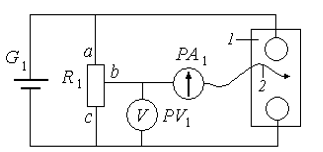
\includegraphics[width=0.9\linewidth]{figures/image.png}
        \label{fig:1.1(1)}
        \caption{Схема установки}
    \end{subfigure}%
    \begin{subfigure}{.5\textwidth}
        \centering
        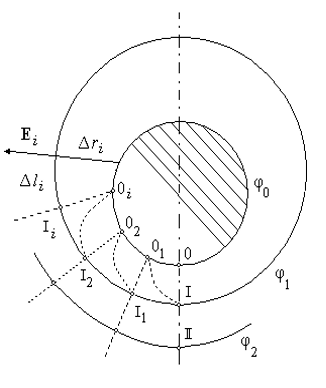
\includegraphics[width=0.7\linewidth]{figures/image2.png}
        \label{fig:1.1(2)}
        \caption{Примерный вид карты поля около одного из электродов}
    \end{subfigure}
\end{figure}

\newpage
$$$$
\newpage
$$$$
\newpage
$$$$

\end{document}